\chapter{Linear Theory}

\section{Introduction}
In this chapter we extend the results of Billant and Chomaz \cite{bc2000c} to the sub-buoyancy length-scales. We also reproduce the numerical results presented by Billant and Chomaz and confirm their conclusions about the existence of the zigzag instability at the buoyancy scale. The results in this chapter are based on the paper by Bovard and Waite \cite{bovard2013}.

\section{Set-up}
The equations that we want to solve are the linear Boussinesq equations, which we derived in Chapter 2 and for which we derived the numerical scheme in Chapter 3. We repeat the equations here:
\begin{align}
\frac{\partial \hat{\bm{u}}}{\partial t} = \textbf{P}(\textbf{k})[\widehat{\bm{u}\times \omega_{z0}\hat{\bm{e}}_{z}} + \widehat{\bm{u}_{h0}\times\bm{\omega}}-\hat{\rho}'\hat{\bm{e}}_{z}] - \frac{k^{2}}{Re}\hat{\bm{u}},\label{solve1}\\
\frac{\partial\hat{\rho}'}{\partial t} = -i\bm{k}_{h}\cdot\widehat{\bm{u}_{h0}\rho'} + \frac{1}{F_{h}^{2}}\hat{w}- \frac{k^{2}}{ScRe}\hat{\rho}'.
\end{align} 
The parameter regime to be explored is a function of $k_{z},Re,F_{h}$. 

In our simulations, we investigate a range of Reynolds numbers $Re=5000-20{,}000$ and Froude numbes $F_{h}=0.05-0.2$. These numbers have been chosen to be within the range of the results of Billant and Chomaz \cite{bc2000c}, who investigated a similar range. This range also falls within potential experimental regimes which could be investigated using the techniques of Billant and Chomaz \cite{bc2000a}. For each $F_{h}$ and $Re$ a wide range of vertical wavenumber, $k_{z}$, were investigated with $k_{z}$ ranging from $1$ to $200$. This wavenumber range incorporates the scale of the zigzag instability down to the viscous damping scale. We additionally consider the Schmidt number to be unity, following the main results of Billant and Chomaz \cite{bc2000c}. In order to compare with experiments, Billant and Chomaz did investigate a non-zero Schmidt number, however their numerical work was dedicated to $Sc=1$ and thus we do not consider different Schmidt numbers here. 

%For certain $Re$ and $F_{h}$, as we shall see below, the viscous damping range changes and thus when the simlations were clearly in the viscous dissipation range, no further simulations were conducted.  We additionally consider the Schmidt number to be unity which is a standard practice (cite... justify? numerically difficult?). 

For our simulations a box size of $L=9$ with $N=512$ grid points was used. The reason for choosing $L=9$ was to minimise interactions of the fields with themselves across the periodic boundary. Lengths of size $L=5$ have been used in practice \cite{augier2012}, however we erred on the side of caution and repeated the box size conditions of Billant and Chomaz \cite{bc2000c}. For robustness results were checked at smaller box size and agree with the tests of \cite{bc2000c}. We used the timesteps of $\Delta t=0.000950$ for $F_{h}=0.2,Re=2000,5000,10000$ and $\Delta t=0.000375$ for all the other simulations. These were chosen following Billant and Chomaz \cite{bc2000c}. 


The code was written in Fortran and all the FFTs were done by FFTW V3.0\cite{fftw} and was tested by comparing the growth rates given by Billant and Chomaz in \cite{bc2000c}, specifically their Figure  1 and Tables 1 and 2. Unlike Billant and Chomaz \cite{bc2000c} we did not restart each simulation with the previous eigenmode because we used a parallel approach for evaluating multiple $k_{z}$ simultaneously. The trade-off is the individual simulations had to be run longer but they could be done in parallel allowing for a greater varability in the parameters explored. 



\section{Growth Rate}
As discussed in Chapter 3, the growth rates are computed by evaluating the time derivative of the energy of the eigenmode. Fig.~\ref{sigma_examples} demonstrates two different types of growth rates that are representative of all the growth rate plots for all the simulations. Here we have chosen $F_{h}=0.1, Re=20{,}000$ and $k_{z}=20$ in panel a and $k_{z}=60$ in panel b. In both panels, the perturbation initially goes through some transient behaviour which is when the various eigenmodes all grow together and none of have become dominant. After about 20 time units this transient behaviour has died off the dominant eigenmode has emerged. This 20 time unit delay was observed for all simulations. In panel (a), there is a case of an oscillatory growth rate. As can be observed, the growth rate of this wavenumber is highly oscillatory and thus the true value of the growth rate must be computed using the period of the oscillatory. Panel (b) represents the more typical case of the growth being non-oscillatory and quickly settling down onto a certain value. 
\begin{figure}
\begin{center}
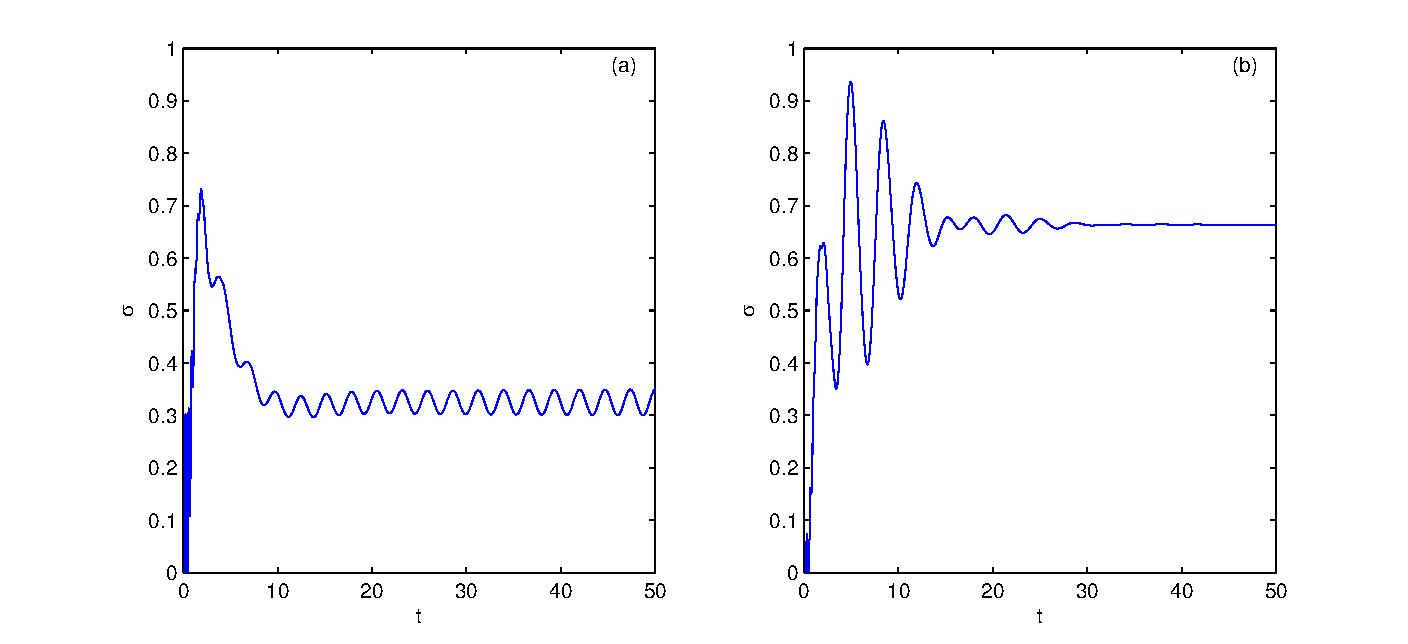
\includegraphics[width=\textwidth]{sigma_examples.pdf}
\caption{Time series of the growth rate, obtained from the derivative of the energy, for $F_{h}=0.1$ and $Re=10{,}000$. Panel (a) is $k_{z}=20$ and Panel (b) is $k_{z}=60$.}
\label{sigma_examples}
\end{center}
\end{figure}

Using these types of plots of the growth rate, we are able to extract the leading growth rate of the maximum eigenmode by examining the long term behaviour. From these times series, we determined the maximum growth rate of the leading eigenmode for a wide range of wavenumbers, Reynolds numbers, and Froude numbers. The growth rate curves for a given $F_{h}$ and $Re$ can be plotted by determining this maximum growth rate for each vertical wavenumber. Following Billant and Chomaz\cite{bc2000c}, we scale the vertical wavenumber by $F_{h}$ to obtain a horizontal scaling $k_{z}F_{h}$.  This is, in our units, scaling by the buoyancy scale $L_{b} = U/N$. Recall that $k_{z}$ has been non-dimensionalised by $R$, i.e. $k_{z}= k_{z}'R$ where $k_{z}'$ is the dimensional wavenumber with units of inverse length. So the dimensionless $F_{h}k_{z}$ would become $F_{h}k'_{z}R$ in dimensional units, $k'_{z}$ denoting the dimensional vertical wavenumber. Re-writing this we obtain $F_{h}k'_{z}R=k_{z}'U/N=k_{z}'L_{b}$, using the definition of the Froude number, and hence dimensional $F_{h}k_{z}'R=k_{z}'L_{b}$ but since $R=1$, $k_{z}'$ and $k_{z}$ have the same value, but with different units. Thus the dimensionless scaling $F_{h}k_{z}$ is like scaling by the buoyancy length. 

\begin{figure}
\begin{center}
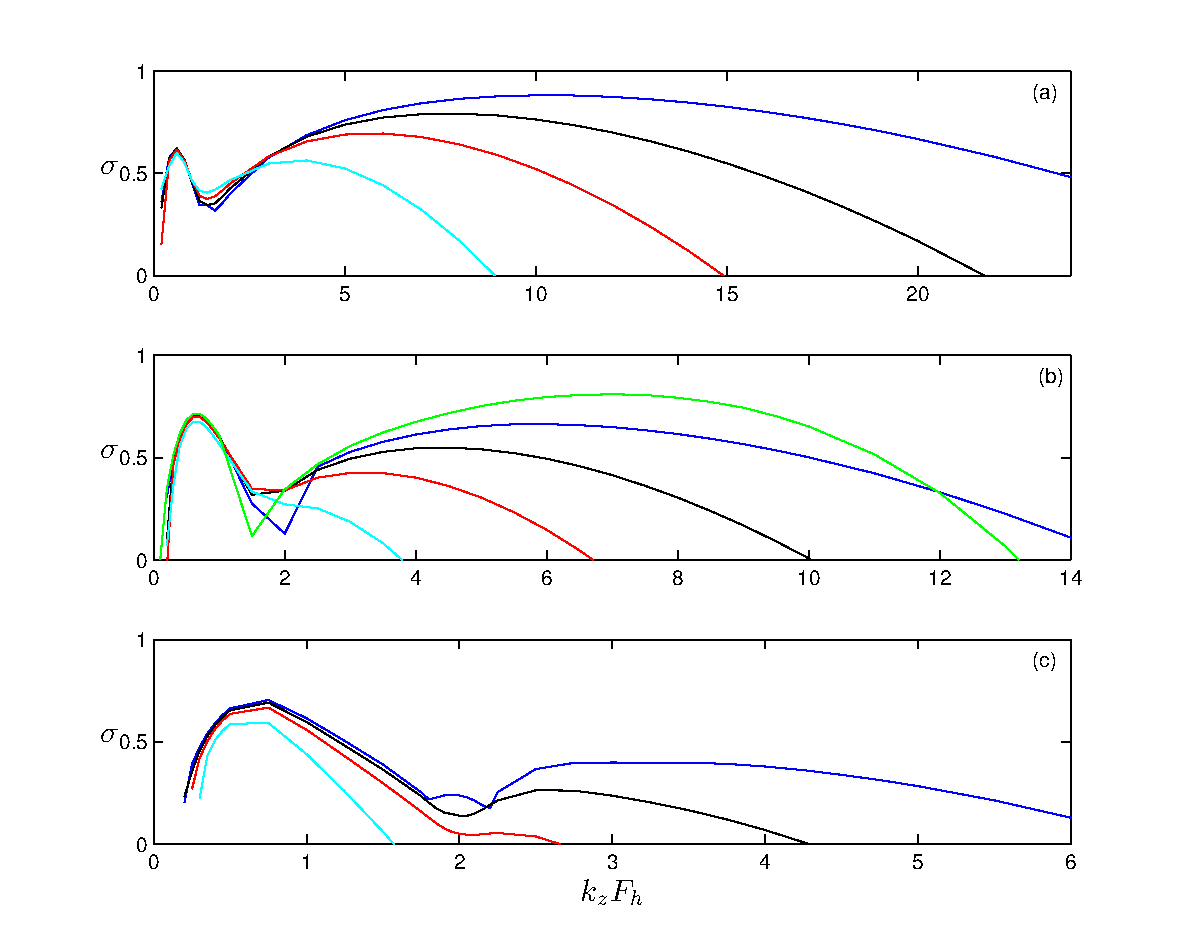
\includegraphics[width=\textwidth]{fixed_froude_varying_reynolds}
\caption{Growth rate $\sigma$ as a function of $k_{z}F_{h}$ for fixed $F_{h}=$(a) $0.2$, (b) $0.1$, (c) $0.05$ with Re$=2000$ (cyan), Re$=5000$ (red), Re$=10000$ (black), Re$=20{,}000$ (blue). In panel (b) the green line is the hyperviscosity case with $Re=20{,}000$.}
\label{FixFhVaryRe}
\end{center}
\end{figure}

Fig.~\ref{FixFhVaryRe} shows the largest eigenmode growth rate as a function of vertical wavenumber for fixed $F_{h}$ and $Re$ for a wide range of $F_{h}$ and $Re$. The qualitative behaviour for the growth rates at different Reynolds numbers are very similar to one another. We now investigate the various regimes in some detail.

At small $F_{h}k_{z}$, the growth rate reaches a local maximum, the zigzag peak, as predicted by Billant and Chomaz \cite{bc2000a,bc2000b,bc2000c}.  As discussed in Chapter 2 the zigzag instability apppears at the buoyancy wavelength $L_{b}$. This is clear from the figure where we can see that peak growth rate occurs at the same $F_{h}k_{z}$, here roughly $F_{h}k_{z}\approx 0.6$. In panels (a) and (b) it is especially clear that the growth rate curves all collapse onto each other and have almost identical growth rates regardless of Reynolds number, confirming the results of the prediction of Billant and Chomaz \cite{bc2000b,bc2000c}. Panel (c) has similar growth rates for $Re=20{,}000,10{,}000,$ and $5000$ but for $Re=2000$ the growth rate is a bit lower. Despite the slight difference in growth rates, they do all occur at the same $k_{z}F_{h}$. The $Re=2000$ case being lower suggests that the diffusion effects are beginning to dominate, as can be seen by the rapid decrease in the growth rate of the curve. Since the theoretical results of Billant and Chomaz \cite{bc2000b} were conduted in an invscid regime, it is not unexpected to observe a breakdown of this assumption. Some numerical experiments were run at even lower Froude number, but here the diffusion was dominating and the growth rate curves were dropping off very rapidly near the zigzag peak and thus even obscurbing the zigzag peak. Thus for $F_{h}<0.05$ and $Re<10{,}000$ we find that the sub-buoyancy length scales are being diffused out. 


For $k_{z}$ increasing beyond the zigzag peak, the growth rate then decreases for increasing $F_{h}k_{z}$ to a local minimum before increasing to a second local maximum. At this local minimum oscillatory growth rates are observed. The imaginary part of the growth rate $\sigma_{i}$ remains zero everywhere else except in this small region between the two local maximum, with the exception of very small $k_{z}F_{h}$. Oscillatory growth rates are also observed in this small regime, as observed in \cite{bc1999} and have been observed before \cite{bc1999} (add in ref 31 of BC1999) and we did not explore this regime. Fig.~\ref{oscillatory_growth} displays the imaginary growth rates for $F_{h}=0.05$ and $Re=10{,}000, 20{,}000$. The imaginary growth rate for $Re=10000$ is a straight line but such a trend is not observed for $Re=20{,}000$. The shape of this curve, when it did appear, depended highly on the Reynold and Froude number, and did not suggest any sort of general result that could be determined about the imaginary growth rate. Additionally, the range of this oscillatory instability also depended on the Froude and Reynolds number and also did not suggest any sort of general result. Due to these observations, we did not explore this regime too closely. 
\begin{figure}
\begin{center}
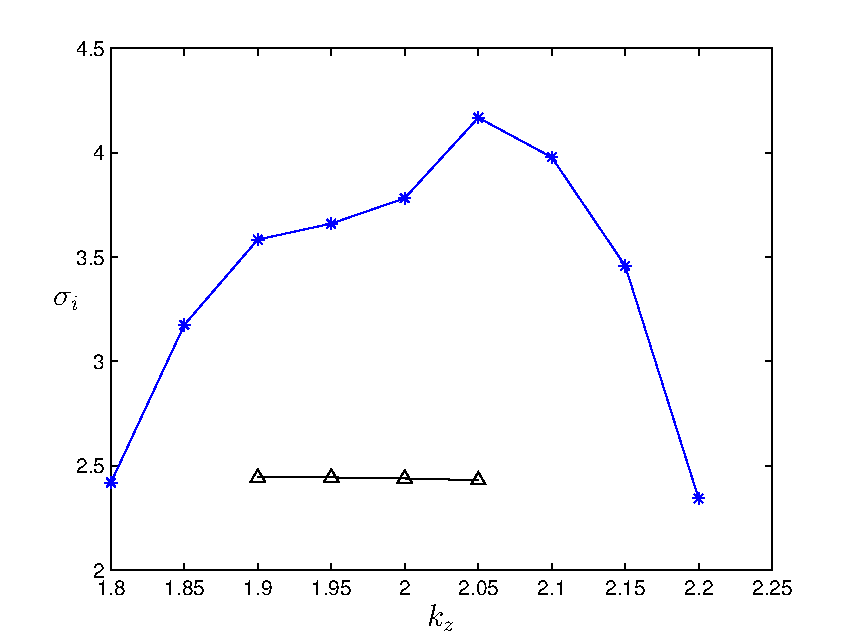
\includegraphics[scale=0.65]{oscillatory_growth}
\caption{Imaginary part of the growth rate for $F_{h}=0.05$ and $Re=20{,}000$ (blue) and $Re=10{,}000$ (black).}
\label{oscillatory_growth}
\end{center}
\end{figure} 

After this local minimum, the growth rate increases to a secondary maximum. We will discuss it further below. Continuing to even smaller vertical scales, viscous effects increase and may damp out the instability, and hence the growth rate decays with increasing $k_{z}F_{h}$ in the limit of large $k_{z}F_{h}$. 

For $F_{h}=0.2$ (Fig.~\ref{FixFhVaryRe}a), the peak growth rate of the short-wave instability exceeds that of the zigzag instability for increasing Reynolds numbers. The growth rates at the second peak is smaller for $F_{h}=0.1$ (Fig.~\ref{FixFhVaryRe}b), but they continue to increase with increasing $Re$. For $F_{h}=0.05$ (Fig.~\ref{FixFhVaryRe}c), the second peak is weaker than the zigzag peak. Fig.~\ref{FixReVaryFh} shows the growth rate for fixed Reynolds numbers with varying Froude numbers. Examining the case of $Re=20{,}000$ (Fig.~\ref{FixReVaryFh}a), the growth rate at the second peak increases with increasing Froude. A similar result is observed for $Re=10000$ and $5000$ (Fig.~\ref{FixReVaryFh}b-c). $Re=2000$ is not included because viscous effects have damped out the second peak in this case. Overall, the dependence of the short-wave growth rate on Froude is also more pronounced than that of Reynolds. For example, the growth rate of the second peak at fixed $Re=20{,}000$ (Fig.~\ref{FixReVaryFh}a) doubles from $F_{h}=0.05$ to $F_{h}=0.2$. By contrast, at fixed $F_{h}=0.2$ (Fig.~\ref{FixFhVaryRe}a), the increase in the growth rate from $Re=5000$ to $Re=20{,}000$ is only about $25\%$ larger. 

\begin{figure}
\begin{center}
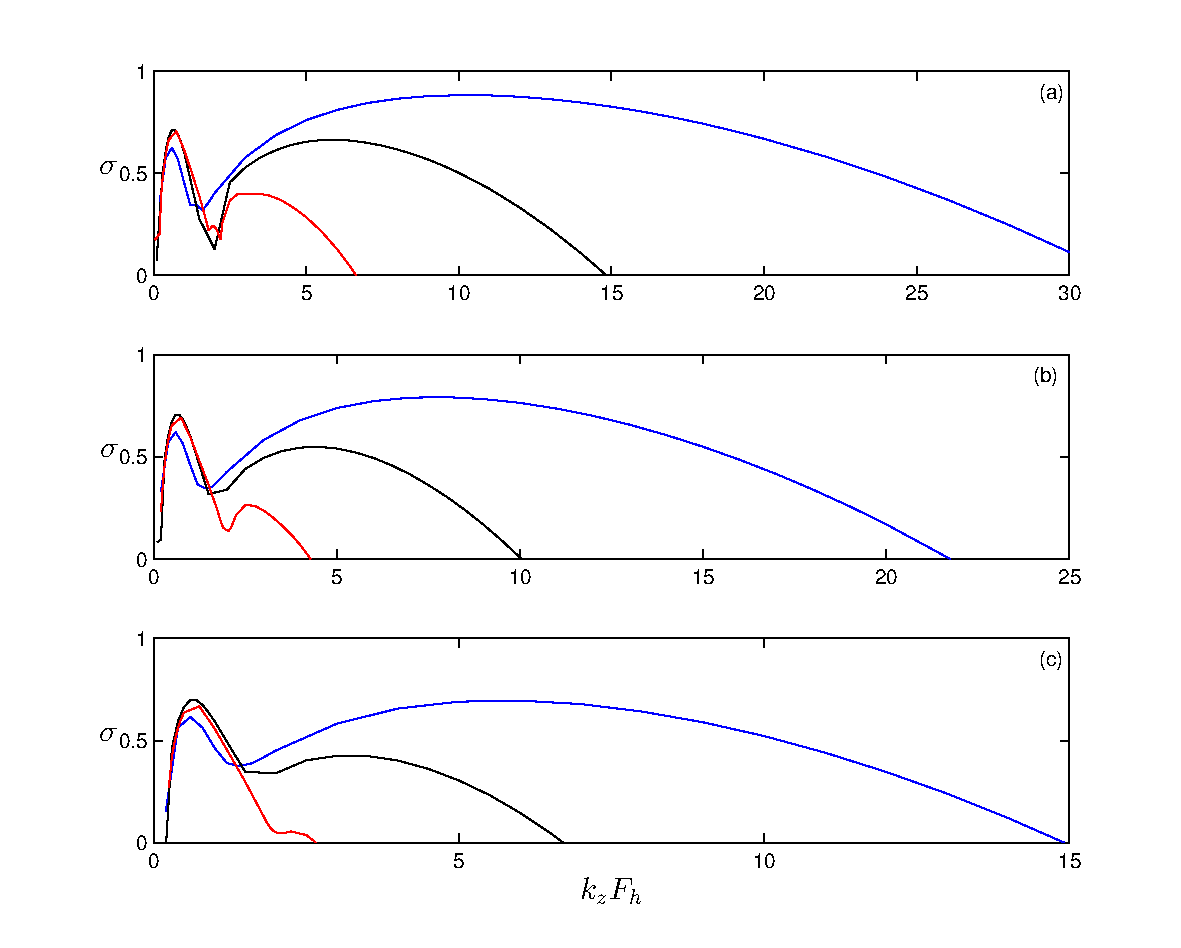
\includegraphics[width=\textwidth]{fixed_reynolds_varying_froude}
\caption{Growth rate $\sigma$ as a function of $k_{z}F_{h}$ for fixed $\text{Re}=(a) 20{,}000, (b) 10000, (c) 5000$ with $F_{h}=0.05$ (red), $F_{h}=0.1$ (black), $F_{h}=0.2$ (blue).}
\label{FixReVaryFh}
\end{center}
\end{figure}
The above analysis demonstrates that the short-wave growth-rate peak moves to larger $k_{z}F_{h}$ with increasing $F_{h}$ and increasing $Re$, but has a stronger dependence on Froude than Reynolds. Some of this joint dependence can be explained by examining the dependence on the buoyancy Reynolds number $Re_{b}=F_{h}^{2}Re$ \cite{riley2003,hebert2006,brethouwer2007}. In stratified turbulence, the buoyancy Reynolds number is analogous to the Reynolds number in the viscous term due to the vertical gradients \cite{brethouwer2007}. As $k_{z}$ increases, we move to smaller vertical scales where the vertical viscosity terms, controlled by the buoyancy Reynolds number, dominates, so it follows that the second peak may be governed by $Re_{b}$. In Fig.~\ref{Buoy} the location of the second peak from Fig.~\ref{FixFhVaryRe} is plotted as a function of the buoyancy Reynolds number. The peak location line is approximately linear and can be fitted with the curve $k_{z}F_{h}= Re_{b}^{2/5}$, which is plotted. This scaling implies that the vertical wavenumber, $k_{z}$, of the short-wave instability is approximately 
\begin{align}
k_{z} \sim F_{h}^{-1/5} Re^{2/5}\label{buoyscale}.
\end{align} 
The dependence of the growth rate on $k_{z}F_{h}$ appears to be similar in the cases with different $F_{h}$ and $Re$ but the same $Re_{b}$. Fig.~\ref{ReBuoy} demonstrates the similarity of the growth rate plotted against $k_{z}F_{h}$ for two cases with $Re_{b}=500$ and two cases with $Re_{b}=50$. For both cases, the locations of the zigzag and second peak line up quite well. The difference between the red and blue curves at the second peak is $4\%$ for $Re_{b}=200$ and $6\%$ for $Re_{b}=50$, a reasonable variation. 

% It is interesting to note that the red curve, corresponding to $Re=20{,}000$ and $F_{h}=0.1$ (a), $F_{h}=0.05$ (b), is lower then the blue curve, corresponding to $Re=5000$ and $F_{h}=0.2$ (a), $F_{h}=0.1$ (b). This supports the observation, and is clear from the definition of the buoyancy Reynolds number, that the stratification may play a more important role in the instability than the viscosity.   

\begin{figure}
\begin{center}
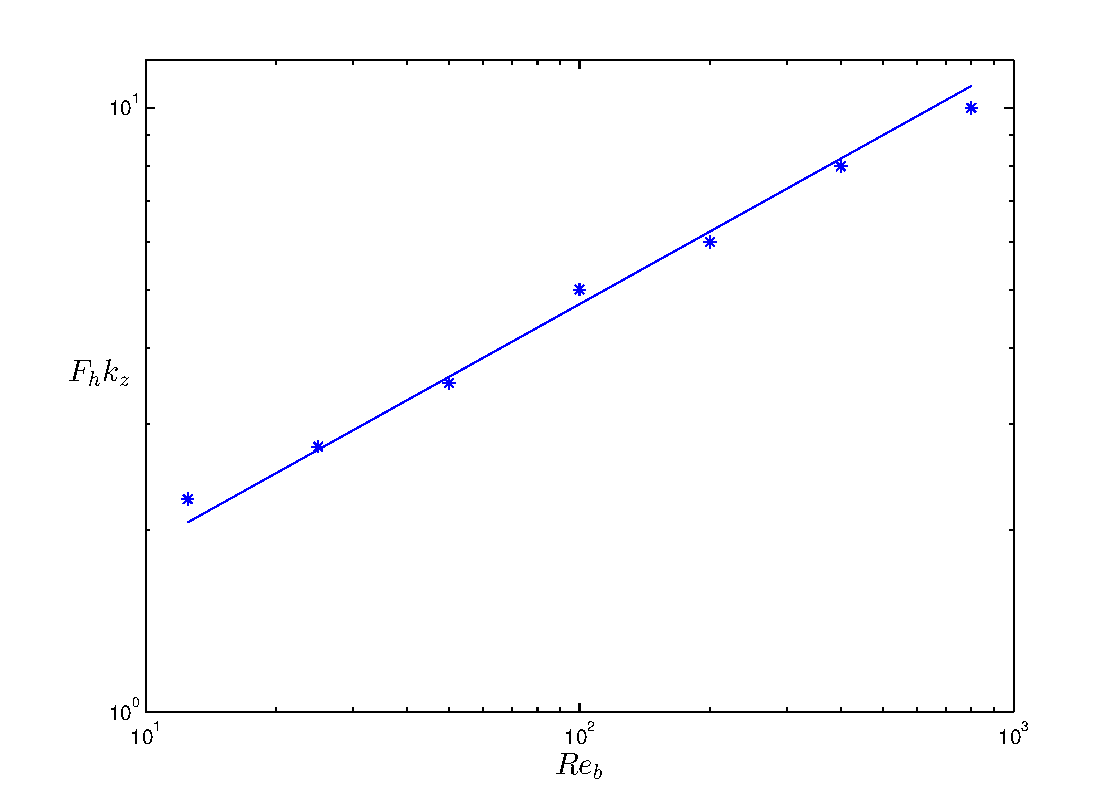
\includegraphics[scale=0.65]{second_peak_buoyancy}
\caption{The location of the second peak as a function of the buoyancy Reynolds number $Re_{b}$. $k_{z}F_{h}$ is taken from Fig.~\ref{FixFhVaryRe}. The straight line is $Re_{b}^{2/5}$.}
\label{Buoy}
\end{center}
\end{figure}
\begin{figure}
\begin{center}
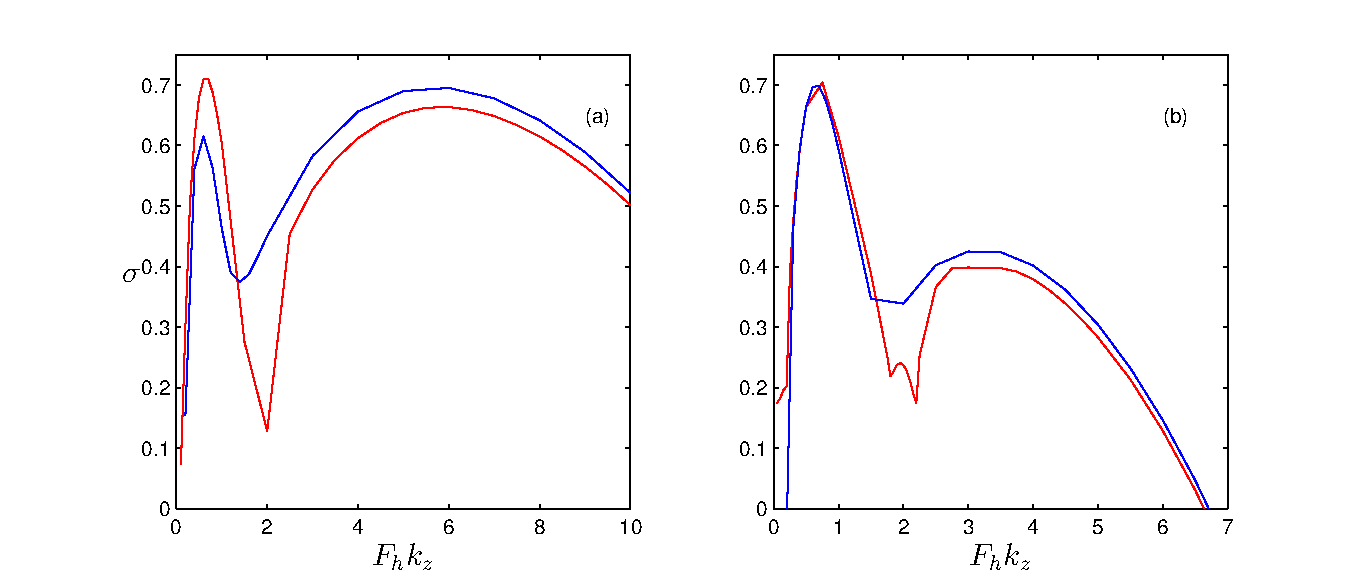
\includegraphics[scale=0.65]{buoyancy_reynolds}
\caption{Growth rate $\sigma$ as a function of $F_{h}k_{z}$ for fixed $Re_{b}$. In (a), red is $Re=20{,}000, F_{h}=0.1$ and blue is $Re=5000, F_{h}=0.2$, both corresponding to $Re_{b}=500$; in (b) red is $Re=20{,}000, F_{h}=0.05$ and blue is $Re=5000, F_{h}=0.1$, both correpsonding to $Re_{b}=50$.}
%\caption{Growth rate $\sigma$ as a function of $k_{z}$ for fixed $Re_{b}=(a) 200, (b) 50$. In (a) red corresponds to $Re=20{,}000, F_{h}=0.1$ blue to $Re=5000, F_{h}=0.2$, in (b) red corresponds to $Re=20{,}000, F_{h}=0.05$, blue $Re=5000, F_{h}=0.1$}
\label{ReBuoy}
\end{center}
\end{figure}


In Fig.~\ref{FixFhVaryRe} (b) the green curve corresponds to a hyperviscosity run with $Re=20{,}000$, which has $Re_{h}=2.8\times 10^{8}$. The motivation for using hyperviscosity is to capture the higher-Reynolds number regime by restricting dissipation to only the largest wavenumbers. As the hyperviscosity run demonstrates, the zigzag peak is independent of Reynolds number and the existence of the peak would be expected at higher Reynolds numbers. For the second peak, we note that the growth rate  of the hyperviscosity run exceeds that of $Re=20{,}000$ for $k_{z}F_{h}>3$ and reaches a maximum around $k_{z}F_{h}=7$. The maximum growth rate in the hyperviscosity case is around $25\%$ larger than the regular viscosity case with $Re=20{,}000$. At $k_{z}F_{h}=12$ we see the hyperviscosity and non-hyperviscosity curves cross. This intersection corresponds to the horizontal wavenumber at which the hyperviscosity damping rate equals the regular viscous damping rate for $Re=20{,}000$. For $k_{z}$ greater than this maximum, the hyperviscosity operator experiences greater damping than the regular viscosity, which can be seen by the sudden drop off of the growth rate. This simulation presents evidence that as $Re\rightarrow \infty$, the growth rate of the second peak will the same order as, or larger than, the growth rate of the zigzag instability. 

\section{Structure} 
Briefly, we discuss the structure of the zigzag instability. Fig.~\ref{zigzag_vorticity} demonstrates the vertical vorticity of the zigzag peak for $F_{h}=0.2,0.1,0.05$ and $Re=20{,}000$. In all vertical vorticity plots that follow, we have normalised the plots so red represents the maximum velocity or vortcity and blue represents the minimum velocity  or vorticity. Since the vorticity field is real, we have chosen the real part. Only $Re=20{,}000$ has been included, see Fig.~\ref{zigzag_fields}, since the structure is nearly identical for $Re=10{,}000$ and $5000$. This confirms the assumption made by Billant and Chomaz \cite{bc2000b} that the zigzag peak emerges at the buoyancy scale $U/N$ independent of $Re$. A detailed study of the structure of the zigzag instability is done by Billant and Chomaz \cite{bc2000c}. 
\begin{figure} 
\begin{center}
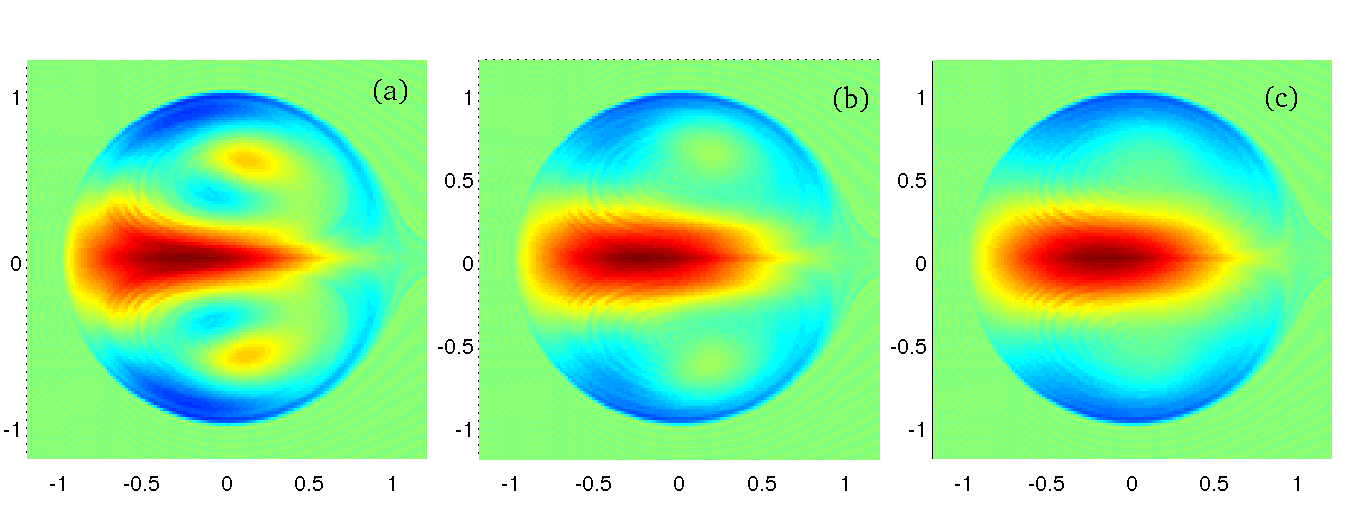
\includegraphics[width=\textwidth]{vorticity_zigzag}
\caption{Perturbation vertical vorticity $\omega_{z}$ at the zigzag peak for $F_{h}=0.2 \text{ (left) }, 0.1 \text{ (middle) }, 0.05 \text{ (right) }$ and $Re=20{,}000$.}
\label{zigzag_vorticity}
\end{center}
\end{figure} 
\begin{figure}
\begin{center}
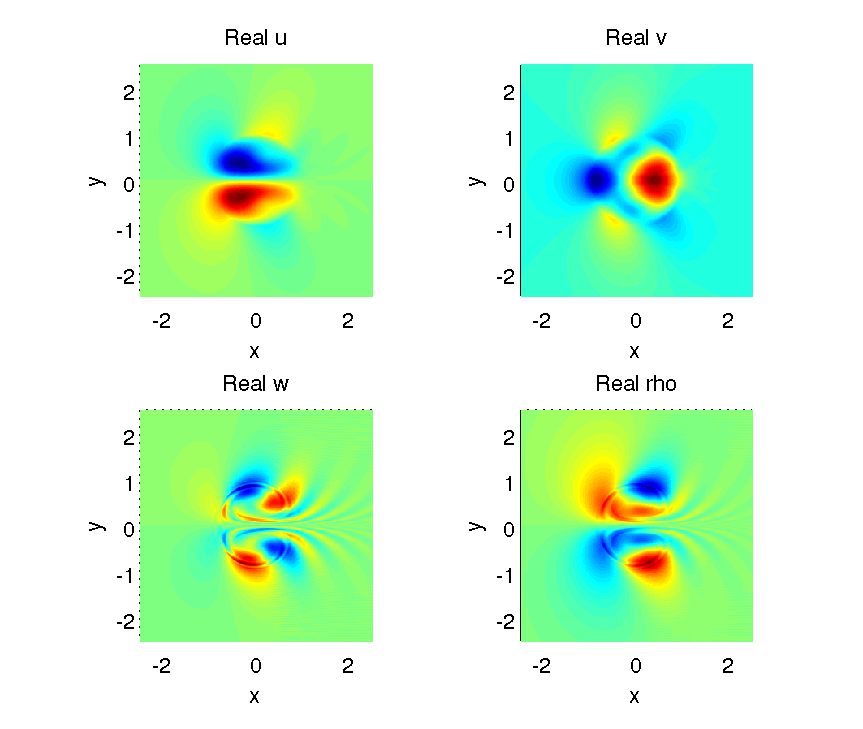
\includegraphics[width=\textwidth]{velocity_fields_kz_6}
\caption{Perturbation fields $u,v,w,\rho$ at the zigzag peak for $F_{h}=0.1$ and $Re=20{,}000$. Here $k_{z}=6$.}
\label{zigzag_fields} 
\end{center}
\end{figure} 

The minimum between the zigzag and short-wave instability is the oscillatory minimum. Fig.~\ref{oscillation_vorticity} and Fig.~\ref{oscillation_fields} are the vorticity and velocity fields respectively. In the vorticity structure, for $Re=20{,}000$ the structure is much more defined then the smoothed out structure of the zigzag instability. At the largest Froude number, the vorticity is in thin strips around the dipole. At the middle Froude number (b),(e),(h) the core of the dipole, new structure has emerged has has a swirl-like pattern. At the smallest Froude number (c),(f),(i), this structure has become much more detailed and a swirl-like pattern has clearly emerged. Additionally, as we increase the viscosity, this swirl-like structure becomes more diffused out. 
\begin{figure}
\begin{center}
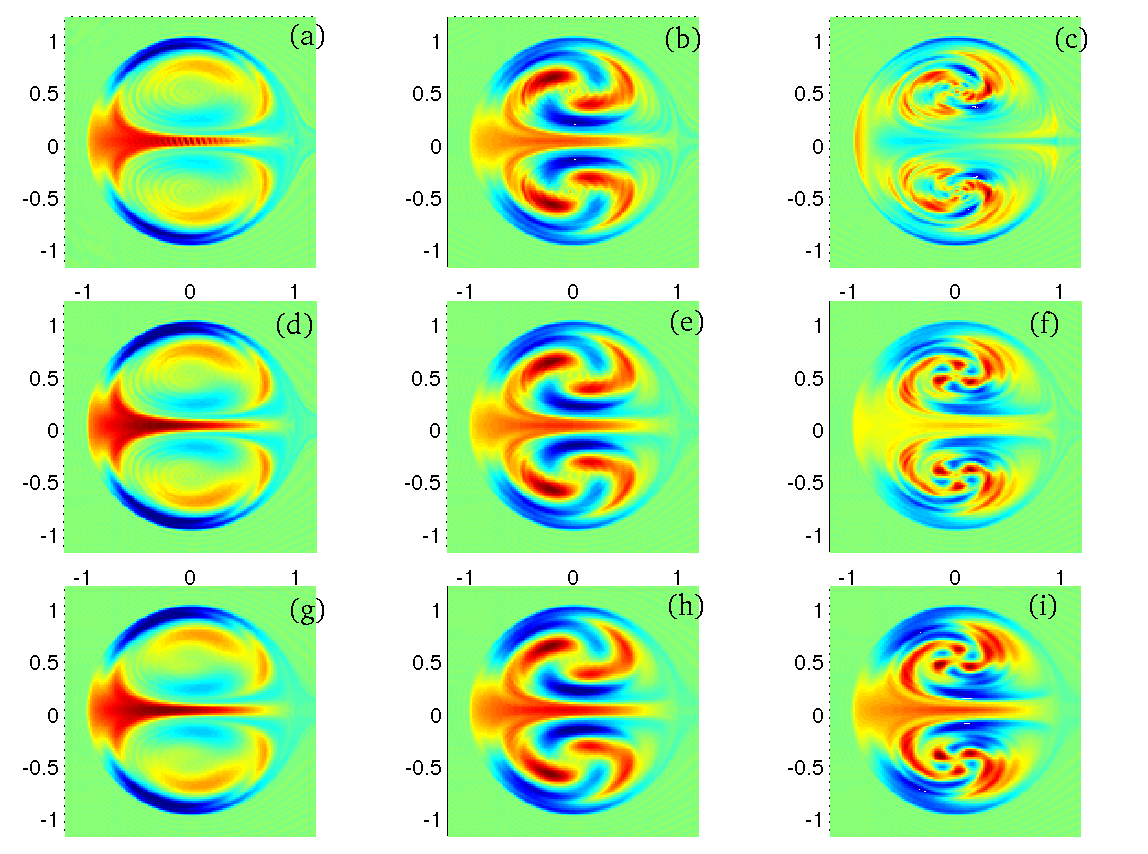
\includegraphics[width=\textwidth]{vorticity_oscillation}
\caption{Perturbation vertical vorticity $\omega_{z}$ at local oscillatory minimum for $Re=20{,}000\text{ (top) }, 10000 \text{ (middle) }, 5000 \text{ (bottom) }$; and $F_{h}=0.2 \text{ (left) }, 0.1 \text{ (middle) }, 0.05 \text{ (right) }$.}
\label{oscillation_vorticity}
\end{center}
\end{figure} 
\begin{figure}
\begin{center}
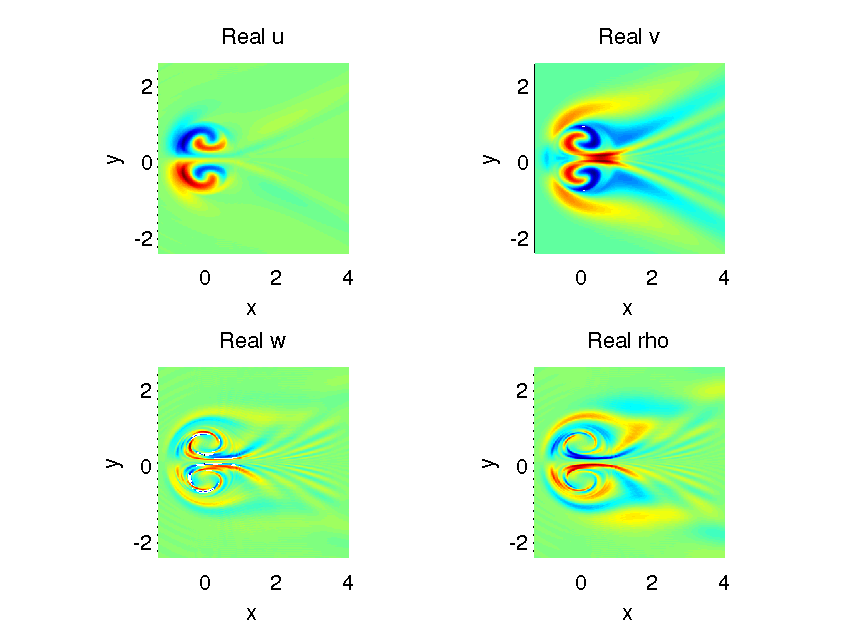
\includegraphics[width=\textwidth]{velocity_fields_kz_20}
\caption{Perturbation fields $u,v,w,\rho$ at the oscillatory minimum for $F_{h}=0.1$ and $Re=20{,}000$. Here $k_{z}=20$.}
\label{oscillation_fields}
\end{center}
\end{figure} 

\begin{figure}
\begin{center}
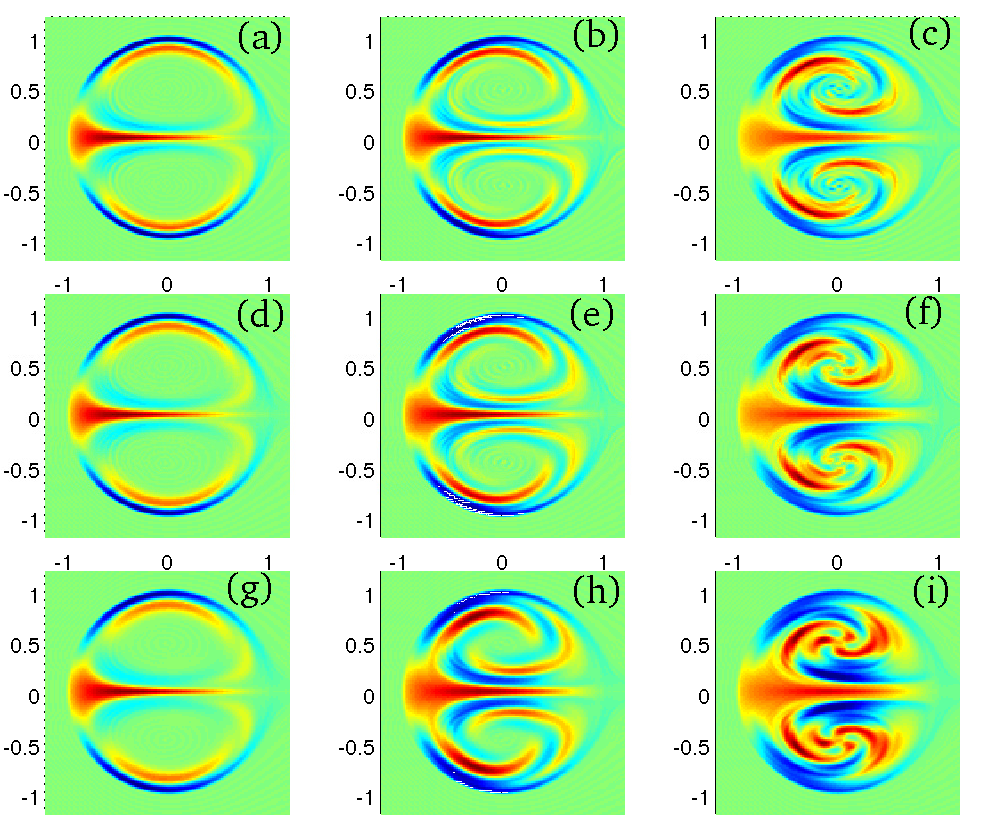
\includegraphics[width=\textwidth]{vorticity_second_peak}
%\caption{Perturbation vertical vorticity $\omega_{z}$ for $k_{z}$ at the second peak. $F_{h}=(a)(d)(g) 0.2 ,(b)(e)(h) 0.1, (c)(f)(i), 0.05, Re=(a)(b)(c) 20{,}000, (d)(e)(f) 10000, (g)(h)(i) 5000$.}
\caption{Perturbation vertical vorticity $\omega_{z}$ at second peak for $Re=20{,}000\text{ (top) }, 10000 \text{ (middle) }, 5000 \text{ (bottom) }$; and $F_{h}=0.2 \text{ (left) }, 0.1 \text{ (middle) }, 0.05 \text{ (right) }$.}
\label{secondpeak}
\end{center}
\end{figure}
\begin{figure}
\begin{center}
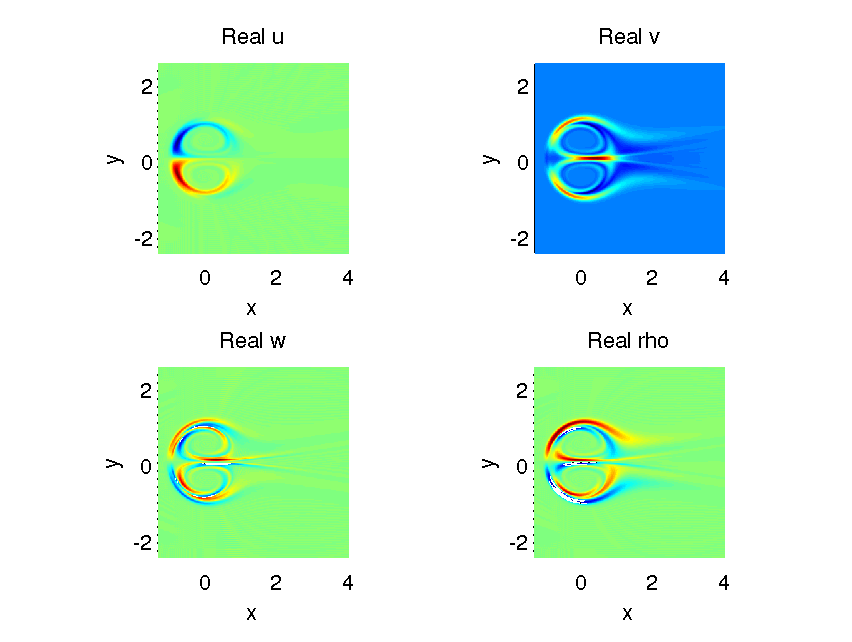
\includegraphics[width=\textwidth]{velocity_fields_kz_60}
\caption{Perturbation fields $u,v,w,\rho$ at the short wave instability for $F_{h}=0.1$ and $Re=20{,}000$. Here $k_{z}=60$.} 
\label{secondpeak_fields}
\end{center}
\end{figure} 
Fig.~\ref{secondpeak} and Fig.~\ref{secondpeak_fields} show the spatial structure of the perturbation vertical vorticity and fields at the second peak for different $Re$ and $F_{h}$. Qualitatively, we observe greater variation for different Froude numbers versus different Reynolds number as suggested above.  At the largest Froude number, the perturbation vorticity is organised in thin strips around and inside the dipole core between the two vortices. Panels (b),(e),(h) have $F_{h}=0.1$ and have a similar overall structure to the larger Froude number. Here, in the cores of the vortices, there is an emergence of a swirl-like pattern. At lower Reynolds number, the structure is spread out due to diffusion, while at higher Reynolds number, small-scale structure is beginning to emerge. This trend continues overall as we move to lower Froude numbers. 

Examining Figs.~\ref{secondpeak} (g)-(i) (fixed $Re$ and decreasing $F_{h}$), the core of the dipoles has a twisting-like behaviour as the Froude number decreases. From this we can conclude that the instability structure of the second peak depends more on the Froude number than on the Reynolds number, which again reinforces the buoyancy Reynolds number scaling.  Indeed, if we consider the cases with $Re_{b}=50$ and $200$ as above, which correspond to Fig.~\ref{secondpeak} (b),(g) and (c),(h) respectively, we can see similar structure in the vorticity fields. Additionally, the anti-symmetric structure of the perturbation can be observed in the dominant eigenmodes in all cases, as found by \cite{bc1999,bc2000c}.

% The vorticity being very thin in the centre is consistent with the results of \cite{pierrehumbert1986} which examined unstratified inviscid vortices at small vertical scales which also demonstrated this behaviour. 
\begin{figure}
\begin{center}
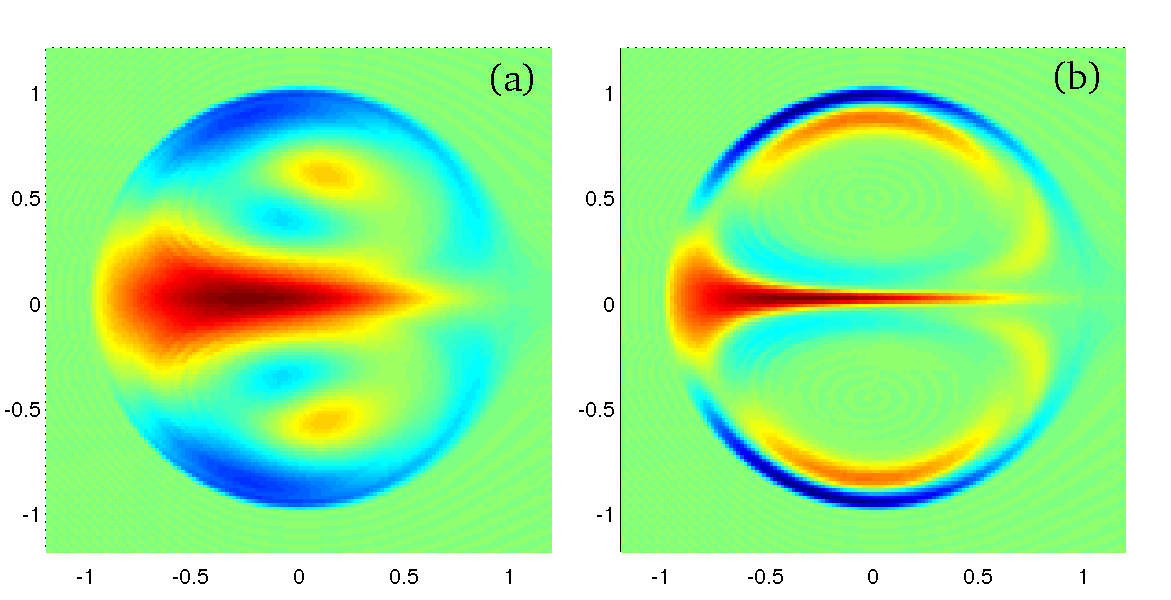
\includegraphics[scale=0.5]{second_peak_vs_zigzag}
\caption{Perturbed vertical vorticity $\omega_{z}$ at (a) the zigzag peak (b) the second peak for $Re=5000, F_{h}=0.2$}
\label{zigzagcomparison}
\end{center}
\end{figure}

Fig.~\ref{zigzagcomparison} shows the perturbation structure for the zigzag peak (a) and the short-wave peak (b) for the case of $Re=5000,F_{h}=0.2$. This case was chosen because the growth rates of the two wavenumbers is roughly the same (see Fig~\ref{FixFhVaryRe} a). The zigzag instability exhibits a quadrupole vorticity structure as discussed in \cite{bc2000c}, which corresponds to a bend and a twist of the basic state dipole. The short-wave instability shares some common overall structure with the zigzag instability. Both have a line of vorticity centred in between two Lamb-Chaplygin vortices and have a ring of vorticity negative vorticity around the outer edges of the dipoles. Additionally, the number of local maximum and minimum remains the same. However, in the short-wave instability, these bands of vorticity have been squeezed into thinner strips and are much more localised along the outer edges of the vortices. In the cores of the dipoles, there is almost no structure and we do not see a quadrupole moment. The full vorticity field of the short-wave instability has a much more dominant twist then the zigzag instability and the bending of the dipole is reduced. As the stratification is increased, this behaviour continues but there is a significant emergence of structure within the cores of the vortices, as observed in Fig~\ref{secondpeak}.


\begin{figure}
\begin{center}
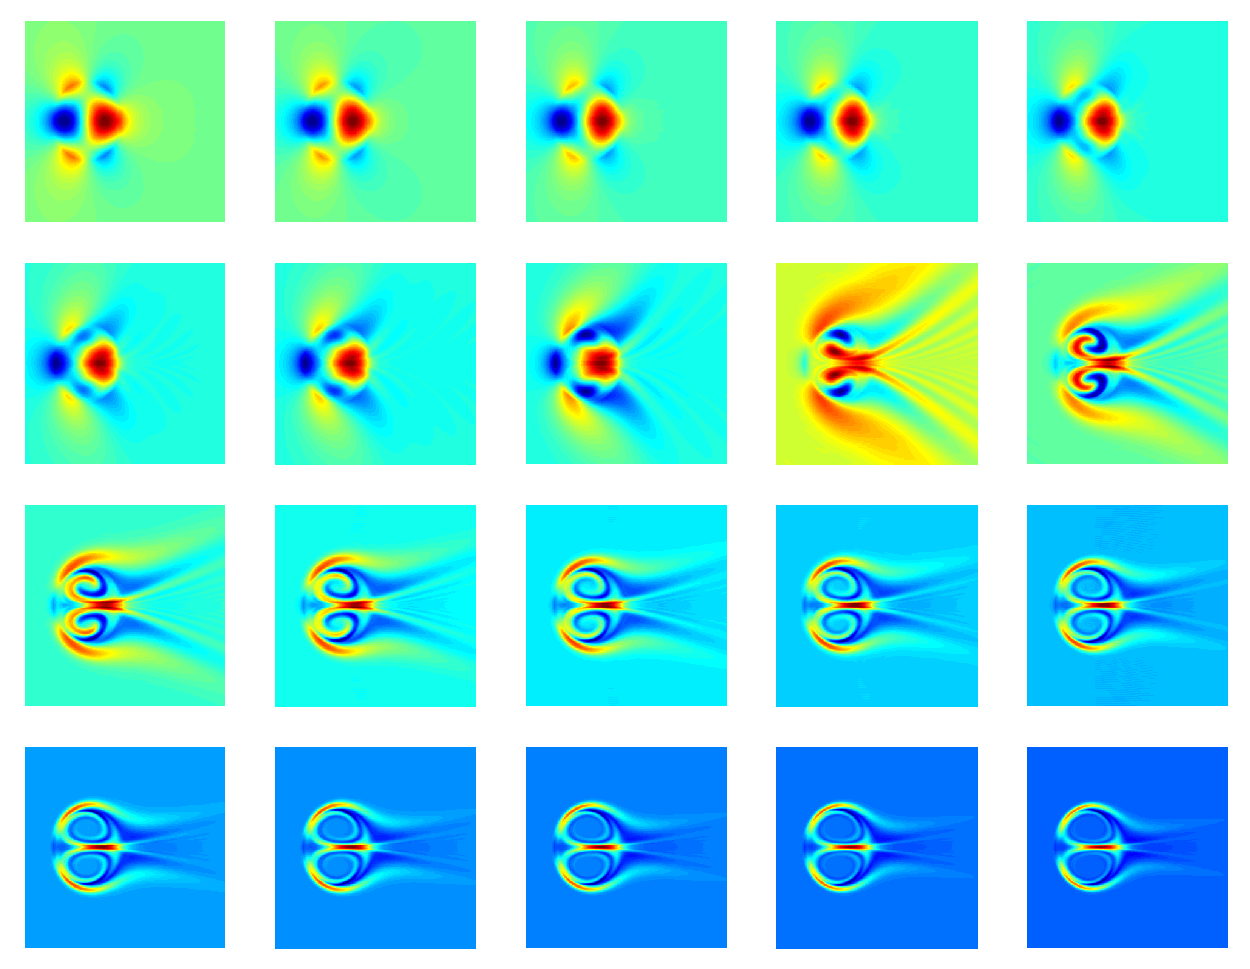
\includegraphics[width=\textwidth]{velocity_field_evolution_u_fh_01_re_20000}
\caption{Structure of the v velocity from $k_{z}=3$ up to $k_{z}=110$ for $F_{h}=0.1$ and $Re=20{,}000$. The wavenumber is increasing left to right and top to bottom. Here the scaling has not been applied to better illustrate the structure.}
\label{evolution}
\end{center}
\end{figure}

Fig.~\ref{evolution} demonstrates the structure of the $v$ component of velocity for $F_{h}=0.1$ and $Re=20{,}000$ for a range of wavenumbers. Here the transition from the zigzag peak, through the oscillatory minimum to the short-wave instability is explicit. Initially the structure has a large positive and negative velocity but as we increase $k_{z}$ this positive velocity is stretched forward and flattened out and becomes stretched out in the middle of the velocity field. The initial negative velocity simply dies out. The initial small areas of positive velocity in front of the dipole undergo an interesting evolution and become larger and stretched out wrapping around the back of the dipole and become very thin. The small initial negative velocity also becomes stretched out but instead forms a v-like shape behind the dipole. The evolution of this wake looks quantitatively similar to the wake of a boat through water. Fig.~\ref{wake} is a loglog plot of the angle of this wake as a function of the perturbation wavelength. The red line is a reference slope of $k=1$ and suggests the relationship between the angle and the wavenumber to be
\begin{align}
\theta \sim \frac{1}{k_{z}}.
\end{align} 
An investigation by Sharman and Wurtele \cite{sharman1983ship} suggests an inverse relationship between the angle of the wake and the vertical wavenumber. However their stratification set-up is different from ours and it is unlikely their analysis carrys over directly, however it does suggest there maybe a similar theory that can be derived for the case of waves behind vortices. 

\begin{figure}
\begin{center}
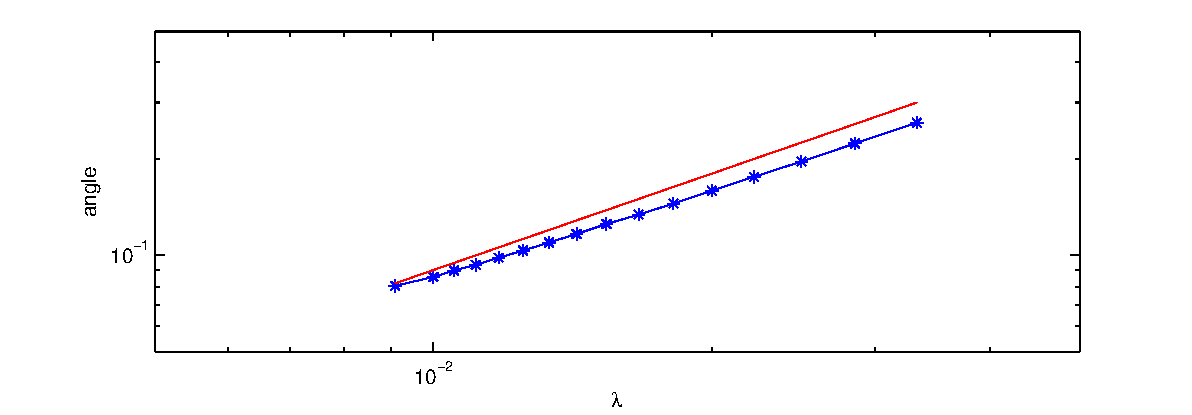
\includegraphics[width=\textwidth]{wake_fh_01_re_20000}
\caption{Angle of the wake behind the v velocity field as a function of the perturbation wavelength for $F_{h}=0.1$ and $Re=20{,}000$. The red line is a reference slope of $1$.}
\label{wake}
\end{center}
\end{figure}

\section{Subdominant modes}
The method we have used so far is limited to only determining the leading eigenmode. An interesting question is whether or not we can determine sub-dominant eigenmodes and what wecan learn from these modes. For example, is the same eigenmode dominating at both the zigzag peak and the short wave peak? To investigate this question, we use a Krylov space method to obtain the growth rates for subdominant modes (cite jet paper). Recall that our linear stability problem can be written as 
\begin{align}
\frac{d\bm{u}}{dt} = A\bm{u}
\end{align}
where $\bm{u}=\bm{u}(\bm{x},t)$ is vector of the unknowns and $A$ is the associated linear operator. We can consider solutions of the form $\bm{u}(\bm{x},t)=\hat{\bm{u}}(\bm{x})e^{\sigma t}$, where $\sigma$ is the growth rate. Plugging in we obtain the following eigenvalue equation for $u$
\begin{align}
\sigma \hat{\bm{u}} = A\hat{\bm{u}}.
\end{align}
As mentioned, we have only been trying to find the leading eigenvalue $\sigma$ but since this is an eigenvalue problem, many algorithms exist to find the eigenspectrum. 

If we want to solve this eigenvalue problem, we must discretise the operator $A$. For our numerical scheme, we do not explicitly construct this operator because it would get very large. Our code is equivalent to this matrix multiplication if one were to write all the FFTs as a matrix multiplication. Writing out operators this way in practice is unfeasible since for our problem, it would require a matrix that is of size $4N^{2}\times 4N^{2}$ and is very dense. Thus trying to find the eigenvalues using a direct eigenvalue routine is not possible. Instead we investigate other algorithms that can determine the eigenvalues without computing $A$ explicitly. 

\subsection{Krylov Eigenvalue Routines}
One of the simplest and easiest to code algorithms for finding eigenvalues is the power method. It is given by the following iteration \cite{MeyerLinAlg}
\begin{align}
u_{k+1}=\frac{Au_{k}}{|Au_{k}|}, \sigma_{k}=\frac{u_{k}^{t}Au_{k}}{u_{k}^{t}u_{k}}.
\end{align}
The reasoning for this algorithm is very simple. If we suppose that the operator $A$ has a spectrum of eigenvalues such that $\lambda_{1} > \lambda_{2} > \ldots $ then by the spectral theorem we can re-write the operator $A$ as
\begin{align}
A = \lambda_{1}\bm{u}_{1}\bm{u}_{1}^{T} + \lambda_{2}\bm{u}_{2}\bm{u}_{2}^{T} + \lambda_{3}\bm{u}_{3}\bm{u}_{3}^{T} + \ldots 
\end{align} 
where $\bm{u}_{i}$ is the eigenvector associated with $\lambda_{i}$. Now recall that by the spectral theorem we have the following \cite{MeyerLinAlg}
\begin{align}
\left(\frac{A}{\lambda_{1}}\right)^{n} = \bm{u}_{1}\bm{u}_{1}^{T} + \left(\frac{\lambda_{2}}{\lambda_{1}}\right)^{n}\bm{u}_{2}\bm{u}_{2}^{T} + \left(\frac{\lambda_{3}}{\lambda_{1}}\right)^{n}\bm{u}_{3}\bm{u}_{3}^{T} + \ldots 
\end{align}
and since there is an ordering on the eigenvalues we have that $\lambda_{i}/\lambda_{1}<1$ and hence as $n\rightarrow\infty$ these terms will vanish. Thus if we consider a random initial vector $\bm{b}_{0}$ we have that 
\begin{align}
\frac{A^{n}\bm{b}_{0}}{\lambda_{1}^{n}}\rightarrow \bm{u}_{1}\bm{u}_{1}^{T}\bm{b}_{0}, n\rightarrow\infty.
\end{align}
Now in practice we don't have $\lambda_{1}$ but if we replace $\lambda_{1}$ with the norm of $|A^{n}\bm{b}_{0}|$ we can still get a good approximation \cite{MeyerLinAlg}. By repeated iteration we obtain the scheme from above. This very simple algorithm is able to give us the leading eigenvalue and eigenvector starting from any random initial vector. A rigorous derivation is contained in any good numerical linear algebra book, e.g. Trefethen and Bau \cite{trefethen1997}.

One drawback of this method is that we are throwing away a lot of information at each iteration. It does not seem unreasonable that maybe these previous approximations can tell us something.Utilising this extra information is the key of Krylov methods. First, we define a Krylov sequence to be 
\begin{align}
\{u,Au,A^{2}u,\ldots,A^{n-1}u\}
\end{align}
This definition is just taking the first $n$ iterations of the power method and defining a sequence of them. Likewise we can also define the Krylov matrix as 
\begin{align}
K_{n}(A,u)=(u|Au|A^{2}u|\ldots|A^{n-1}u)
\end{align}
where we are defining a new matrix whose $i$th column is the $i$ iteration. This Krylov matrix allows us to compute the sub-dominant modes.  

Consider the following matrix, $L=K^{-1}AK$, which is the similarity transformation of $A$ by $K$. Recall that the eigenvalues of similar matrices are the same \cite{MeyerLinAlg}. This is the key idea of the Krylov methods, if we apply a similarity transform to our original matrix $A$ by $K$ we can instead compute the eigenvalues of $L$. However we still are stuck with the inverse matrix $K^{-1}$. To compute this inverse, we orthogonalise $K$ (by Gram-Schmidt) and thus $K^{-1}=K^{t}$. 

So far everything has been exact since the size of $K$ must be the same size as $A$. Now we make the approximation that we can replace $K$ with $K_{n}$. Now taking the first $n$ iterations, and $n$ being small in some sense, let us define a new matrix $P$ as above
\begin{align}
P=K_{n}^{t}AK_{n}.
\end{align}
Now $P$ is no longer the same size as $A$. Clearly the similarity properties no longer hold but if the eigenvalues of $P$ are computed, they, rather amazingly, turn out to be a very good approximation to $A$. This leads to a very simple idea for finding dominant eigenvalues for A: simply choose a small $n$ and then find the eigenvalues of $P$ which is only $n\times n$ and there exist many good algorithms for finding the eigenvalues of small $n$. 

This amazing fact has been fairly well understood for symmetric $A$ and leads to the Lanczos algorithm \cite{MeyerLinAlg} (Krylov book). The non-symmetric case is less well understood and leads to the Arnoldi iteration. Similar ideas of using Krylov sequences and matrices form the theoretical basis for conjugate gradient and GMRES algorithms for solving linear systems.  


\subsection{Results}
\begin{figure}
\begin{center}
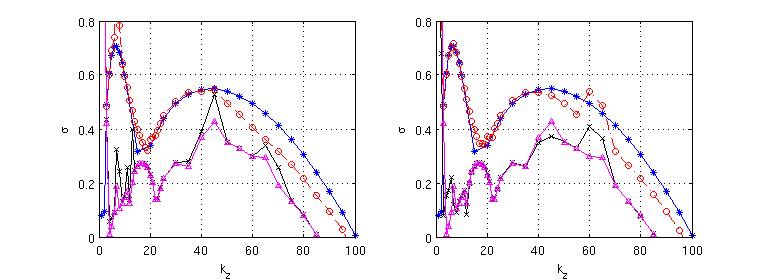
\includegraphics[scale=0.7]{final_data.png}
\caption{Krylov methods with two different choices of $n=50$  (left), $100$ (right) for $Re=10000, N=256, F_{h}=0.1$. Star denotes the dominant eigenvalues from the energy method, circle is the leading approximation from the Krylov method, triangle and x are the second and third eigenvalues respectively.}
\label{krylov_tests}
\end{center} 
\end{figure}
Fig.~\ref{krylov_tests} uses the Krylov method for finding sub dominant eigenvalues for the linear stability of a Lamb-Chaplygin dipole in a stratified fluid for $Re=10000, F_{h}=0.1, N=256$. The reason $N=256$ was chosen was for memory issues in MATLAB. Some tests of various sizes of $N$ showed some robustness although a thorough convergence investigation was not completed and the results were only compared to those of the previous sections. To find the Krylov sequence, the output from the simulation of the previous section was saved at certain times.  Selecting $n$ samples, they were orthogonalised using a Gram-Schmidt procedure  and used to form the Krylov matrix $K$. To evaluate $AK$ the linear code was simulated as normal and reformatted into a giant vector. Then $P$ was constructed and the eigenvalues of the resulting matrix were found using MATLAB's \texttt{eigs} routine. 

The results of Fig.~\ref{krylov_tests} are somewhat promising. As can be seen, doubling $n$ does improve convergence, althought there are still numerical anomolies, such as the random jump in growth rate at $k_{z}=60,65$ for $n=100$. As mentioned above, the theory of Krylov methods for non-symmetric matrices is still not well developed and few rigorous results on errors have been derived. The leading eigenvalue is reproduced accurately up to just about the short-wave peak before the Krylov results decay faster. The most promising result is at the local minimum between the two peaks. Here there is a very smooth curve of the growth rates of the second and third eigenmodes whose values are close to the values of the leading eigenmode. This result suggests that at this local minimum, a different eigenmode might be the dominate eigenmode for the short wave instability than that of the zigzag peak. Returning to the structure, Fig.~\ref{evolution} supports this viewpoint as the the zigzag and short-wave peak velocity fields are different and the oscillatory region in between suggests a combination of the two which might be the two different modes interchanging dominance and resulting in a mix of the two. 

Finally, some attempts were made use MATLABs \texttt{eigs} routine and passing the operator $A$ explicitly, instead of evaluating from a time series, were unsuccesful despite many hours of debugging. 

\section{Dimensional Analysis}
Motivated by the scale analysis of those presented in the Chapter 2 review \cite{lilly1983,rileylelong2000,bc2001,brethouwer2007}, we present a scaling analysis for small vertical scales as considered in the above numerical simulations. We consider the Boussinesq equations

\begin{align}
\frac{\partial \textbf{u}_{h}'}{\partial t'} + \textbf{u}_{h}'\cdot\nabla'_{h}\textbf{u}_{h}'+u_{z}'\frac{\partial \textbf{u}_{h}'}{\partial z'} &= -\frac{1}{\rho_{0}}\nabla'_{h}p' + \nu \nabla'^{2}\textbf{u}_{h}\label{scaling_horz},\\
\frac{\partial u_{z}'}{\partial t'} + \textbf{u}_{h}'\cdot\nabla'_{h}u_{z}'+u_{z}'\frac{\partial u_{z}'}{\partial z'} &= -\frac{1}{\rho_{0}}\frac{\partial p'}{\partial z'} - \frac{\rho' g}{\rho_{0}} + \nu \nabla'^{2}u_{z},\label{scaling_vert}\\
\nabla'_{h}\cdot\textbf{u}_{h}' + \frac{\partial u_{z}'}{\partial z'} &=0,\label{scaling_cont}\\
\frac{\partial \rho'}{\partial t'} + \textbf{u}_{h}'\cdot\nabla_{h}'\rho' + u_{z}'\frac{\partial \rho'}{\partial z'} + \frac{\partial \rho}{\partial z'}u_{z}'&=D\nabla^{2}\rho ',\label{scaling_moment}
\end{align}
where the primed notation denotes the dimensional variables in this section only. 

Following \cite{bc2001} let $U,W$ be the characteristic velocities in the horizontal and vertical directions, $L_{h},L_{v}$ be the corresponding characteristic length scales, $P$ be the pressure, and $R$ be density perturbation scales, not to be confused with the dipole radius $R$ from above. We assume, differing from the analysis of \cite{lilly1983,bc2001}, that in addition to $U,L_{h}$ being imposed on the system, we also impose a separate vertical scale $L_{v}$. This scaling is motivated by the above numerical simulations where we impose a vertical length scale through the vertical wavenumber $k_{z}$. The aspect ratio $\delta=L_{v}/L_{h}$ is assumed to be small, i.e. $\delta<1$. We define the horizontal Froude number to be $F_{h}=U/NL_{h}$, which is also assumed to be small. Following the above numerical simulations, let $\delta < F_{h}$, which we can also write as $L_{v} < U/N$, i.e. vertical scales are assumed to be smaller than the buoyancy scale. We now define the advective time scale $T=L_{h}/U$. 
To determine the characteristic scale of $W$, we are left with two choices: imposing the scaling from the continuity equation or from the density equation. Previous work \cite{bc2001} chose the latter and obtained a characteristic velocity 
\begin{align}
W \lesssim \frac{RF_{h}g}{\rho_{0}N}\label{scaling1}. 
\end{align}
By contrast, we use the continuity equation (\ref{scaling_cont}), which implies
\begin{align}
W \lesssim \delta U\label{scaling2}.
\end{align}
This scaling for $w$ is consistent with the assumption that $\delta < F_{h}$. Using (\ref{scaling2}), the vertical momentum equation (\ref{scaling_vert}) gives a density scaling of $R\sim \rho_{0}U^{2}/(gL_{v})$. Plugging this result into (\ref{scaling1}), we obtain $W\sim UF_{h}^{2}/\delta$. Because $\delta < F_{h}$ we have $U\delta < UF_{h}^{2}/\delta$ so our assumptions are consistent. Setting $W\sim U\delta$ the horizontal momentum equation (\ref{scaling_horz}) gives $P\sim \rho_{0}U^{2}$. Combining this all, we obtain the following scaling for the Boussinesq equations with $L_{v} < U/N$:  

\begin{align}
\textbf{u}_{h}' = U\textbf{u}_{h},\qquad u_{z}'=U\delta u_{z},\qquad \rho' =\frac{U^{2}\rho_{0}}{gL_{v}}\rho,\qquad p'=\rho_{0}U^{2}p, \nonumber\\
\textbf{x}=L_{h}x,\qquad z'=L_{v}z,\qquad t' = \frac{L_{h}}{U}{t},\qquad Re=\frac{UL_{h}}{\nu},\qquad Sc = \frac{\nu}{D}
\end{align} 
which leads to  
\begin{align}
\frac{\partial \textbf{u}_{h}}{\partial t} + \textbf{u}_{h}\cdot\nabla_{h}\textbf{u}_{h}+u_{z}\frac{\partial \textbf{u}_{h}}{\partial z} &= -\nabla_{h}p + \frac{1}{Re}\nabla_{h}^{2}\textbf{u}_{h} +  \frac{1}{\delta^{2}Re}\frac{\partial^{2}\textbf{u}_{h}}{\partial z^{2}},\\
\delta^{2}\left(\frac{\partial u_{z}}{\partial t} + \textbf{u}_{h}\cdot\nabla_{h}u_{z}+u_{z}\frac{\partial u_{z}}{\partial z}\right) &= -\frac{\partial p}{\partial z} - \rho' + \frac{\delta^{2}}{Re}\nabla_{h}^{2}u_{z} + \frac{1}{Re}\frac{\partial^{2}u_{z}}{\partial z^{2}},\\
\nabla_{h}\cdot\textbf{u}_{h} + \frac{\partial u_{z}}{\partial z} &=0,\\
\frac{\partial \rho'}{\partial t} + \textbf{u}_{h}\cdot\nabla_{h}\rho' + u_{z}\frac{\partial \rho'}{\partial z} -\frac{\delta^{2}}{F_{h}^{2}}u_{z}&=\frac{1}{ReSc}\nabla_{h}^{2}\rho + \frac{1}{\delta^{2}ReSc}\frac{\partial^{2}\rho}{\partial z^{2}},
\end{align}
which holds when $\delta<F_{h}\ll 1$. This suggests that for very small vertical scales with $\delta \ll  F_{h}$ the effects of stratification should be negligible. At such small vertical scales, density variation due to stratification would be negligible and thus we would not expect stratification to play an important role in the overall evolution. Additionally, the presence of the factors of $\delta$ in the denominator of the vertical viscous terms suggests that the effects of viscosity become more dominant at very small vertical scales.  

As a result of this scaling analysis we expect that the nature of the instability at short vertical scales to become independent of $F_{h}$ for large $k_{z}$. To test this hypothesis Fig.~\ref{sigma_scaling} shows growth rate as a function of $k_{z}$ for four sets of simulation with $Re=10{,}000$: $F_{h}=0.2,0.1,0.05$ and a new unstratified case with $F_{h}=\infty$ (note that, unlike in Fig.~\ref{FixReVaryFh}, we are not scaling $k_{z}$ by $F_{h}$). The growth rate curves appear to be converging for large $k_{z}$ where $\delta \ll F_{h}$, which agrees with the conclusion of the above scaling analysis. These large $k_{z}$ are well into the viscous damping range and as discussed above, the effects of viscosity become stronger and we observe a sharper decrease in the growth rate.

For the short-wave instability examined above, $\delta/F_{h}=1/(k_{z}F_{h})$ ranges from $\approx 0.5$ down to $0.1$, which is $<1$ but not $\ll 1$. As a result, we do not necessarily expect the characteristics of this instability to be independent of $F_{h}$ for the parameters considered here. Indeed, our stability analysis shows that the (unscaled) wavenumber $k_{z}$ of the short-wave peak is weakly dependent on $F_{h}$, through the $F_{h}^{1/5}$ factor in (\ref{buoyscale}). However, by examining even larger $k_{z}F_{h}$ (i.e. even smaller $\delta/F_{h}$), this scale analysis suggests that the nature of the short-wave instability will eventually become independent of $F_{h}$.  

\begin{figure}
\begin{center}
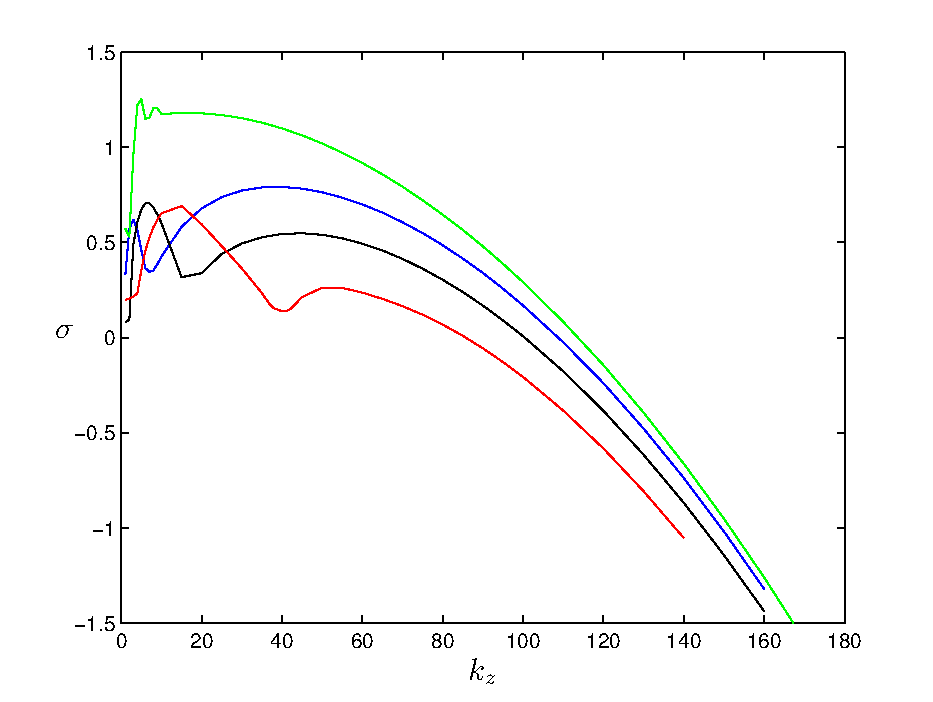
\includegraphics[scale=0.7]{sigma_kz_scaling}
\caption{Growth rate $\sigma$ as a function $k_{z}$ at $Re=10{,}000$ with $F_{h}=\infty$ (green), $F_{h}=0.2$ (blue), $F_{h}=0.1$ (black), $F_{h}=0.05$ (red)}
\label{sigma_scaling}
\end{center}
\end{figure}


